%! Tex Root = edp.tex
\documentclass[../edp.tex]{subfiles}

\begin{document}

{\scshape \hfill 09 de mayo, 2023}

\subsection{Fórmula del Valor Medio}

\begin{wrapfigure}{r}{0.3\textwidth}
	\centering
	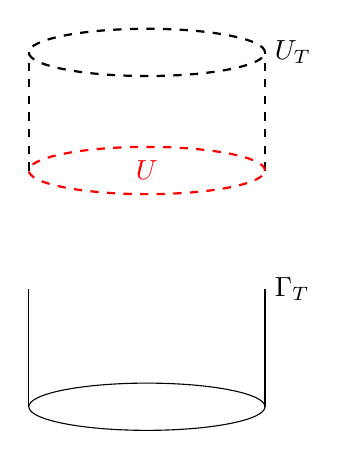
\begin{tikzpicture}[scale=1.5]
		\begin{scope}
			\draw[thick,dashed] (0,1) circle(1 and 0.2);
			\draw[thick,dashed] (-1,0) -- (-1,1);
			\draw[thick,dashed] (1,0) -- (1,1);
			\node[right] at (1,1) {\(U_{T}\)};
			\draw[thick,dashed,red] (0,0) circle(1 and 0.2);
			\node[red] at (0,0) {\(U\)};
		\end{scope}
		\begin{scope}[yshift=-2cm]
			\draw (0,0) circle(1 and 0.2);
			\draw (-1,0) -- (-1,1);
			\draw (1,0) -- (1,1);
			\node[right] at (1,1) {\(\Gamma_{T}\)};
		\end{scope}
	\end{tikzpicture}
\end{wrapfigure}
\begin{Definicion}[Cilindro y Bola de calor]
	Sea \(U\) abierto y acotado en \(\R^n\) y sea \(T > 0\) fijo.
	Definimos:
	\begin{enumerate}[topsep=5pt,itemsep=2pt]
		\item El cilindro parabólico
		\begin{displaymath}
			U_{T} \coloneqq (0,T] \times U;
		\end{displaymath}
		\item La frontera parabólica
		\begin{displaymath}
			\Gamma_{T} \coloneqq \overline{U_{T}} - U_{T};
		\end{displaymath}
		\item Y la bola de calor
		\begin{displaymath}
			W_{r}(t_0, x_0) 
			\coloneqq 
			\left\{
				(t,x) \colon
				t < t_0 \land \Phi(t_0 - t, x_0 - x) > r^{-n}	
			\right\}
		\end{displaymath}
		donde \((t_0, x_0) \in \R\times\R^n\) y \(r > 0\).
	\end{enumerate}
\end{Definicion}

Algunas observaciones sobre la bola de calor. Primero, notemos que
\((t_0, x_0) \in \partial W_{r}(t_0, x_0)\). De hecho,
tenemos que
\begin{displaymath}
	\partial W_r(t_0,x_0) \cap \lbrace0\rbrace\times\R^n
	= \left\{ (t_0,x_0) \right\}.
\end{displaymath}
Por otro lado, la condición sobre \(\Phi\) nos dice que
\begin{displaymath}
	\Phi(t_0 - t, x_0 - x) > r^{-n}	
	\iff
	\frac{1}{\sqrt{4\pi(t_0 - t)}^n} 
	\exp \left(- \frac{\abs{x_0 - x}^2}{4\abs{t_0 - t}}\right)
	> \frac{1}{r^n}
\end{displaymath}
Dado que la exponencial está acotada por \(1\), nos queda la
siguiente estimación:
\begin{displaymath}
	\frac{1}{\sqrt{4\pi(t_0 - t)}^n} 
	> \frac{1}{r^n}
	\iff
	t > t_0 - \frac{r^2}{4\pi}.
\end{displaymath}
Así que, si \((t,x)\in W_r(t_0,x_0)\), entonces \(t \in
(t_0 - \frac{r^2}{4\pi}, t_0) = I\). Esto nos dice que en la bola de calor
no nos podemos ir tan atrás en el tiempo. Cabe preguntarse cómo se
comporta el espacio en este trozo de tiempo \(I\); Para investigarlo, 
tomemos \(s\in I\). Luego, 
\begin{displaymath}
	W_r(t_0,x_0) \cap \lbrace s\rbrace \times\R^n
\end{displaymath}
es una bola (en el espacio) centrada en \((t_0,x_0)\). En efecto,
\begin{align*}
	\Phi(t_0 - s, x_0 - x) > r^{-n}	
	&\iff
	\frac{1}{\sqrt{4\pi(t_0 - s})^n} 
	\exp \left(- \frac{\abs{x_0 - x}^2}{4\abs{t_0 - s}}\right)
	> \frac{1}{r^n}
	\\&\iff
	\left( \frac{r}{\sqrt{4\pi(t_0 - s)}} \right)^n
	>
	\exp \left(\frac{\abs{x_0 - x}^2}{4\abs{t_0 - s}}\right)
	\\&\iff
	\abs{x_0-x}^2
	< 
	4\abs{t_0 - s} n 
	\log \left( \frac{r}{\sqrt{4\pi(t_0 - s)}} \right)
	\eqqcolon \rho(s)^2.
\end{align*}
Luego, \(\abs{x-x_0} \leq \rho(s)\). Nótese que para \(s\uparrow t_0\) y
en \(s \downarrow t_0 - \frac{r^2}{4\pi}\) se tiene que \(\rho(s) \to 0\).
Más aún, a medida que \(s\) disminuye desde \(t_0\) la cota
\(\rho(s)\) crece y luego decrece hasta llegar a \(s = t_0 -
\frac{r^2}{4\pi}\), donde se anula.

Otras observaciones de la bola de calor incluyen:
\begin{enumerate}[itemsep=2pt,topsep=3pt]
	\item Monotonía: Si \(r_1 < r_2\), entonces \(W_{r_1} < W_{r_2}\);
	\item Traslación: \(W_{r}(t_0,x_0) = (t_0, x_0) + W_r(0,0)\);
	\item Dilatación: Si \((t,x) \in W_r(0,0)\) entonces 
	\((t/r^2, x/r) \in W_{1}(0,0)\);
	\item Para \(t_0=0\) y \(x_0=0\), si \(t\in (-r^2/4\pi, 0)\)
	entonces
	\begin{displaymath}
		\Phi(-t, -x) > \frac{1}{r^n}
		\iff
		\frac{\abs{x}^2}{4t} 
		> n 
		\log\left(\frac{-\sqrt{4\pi t}}{r}\right).
	\end{displaymath}
	Definiendo \(b_r\colon \R^{-}\times\R^n \to \R\) mediante
	\begin{displaymath}
		b_r(t,x)
		=
		\frac{\abs{x}^2}{4t}
		+ n\log(r)
		- \frac{n}{2} \log(-4\pi t),
	\end{displaymath}
	tenemos que
	\begin{align*}
		W_{r}(0,0)
		&=
		\left\{
			(t,x) \in \R^{-}\times\R^n\colon
			b_r(t,x) > 0	
		\right\}
		\\	
		\partial W_{r}(0,0)
		&=
		\left\{
			(t,x) \in \R^{-}\times\R^n\colon
			b_r(t,x) = 0
		\right\}.
	\end{align*}
	\item 
	\begin{displaymath}
		\frac{1}{4r^r}
		\int_{W_r(0,0)} \frac{\abs{x}^2}{t^2}\, d(t,x)
		=
		\frac{1}{4}
		\int_{W_{1}(0,0)} \frac{\abs{x}^2}{t^2}\, d(t,x)
		= 1.
	\end{displaymath}
\end{enumerate}

\begin{Proposicion}
	Sean \(R>0\) y \(u\in \CC^{(1,2)}(W_r(0,0))\). Definiendo
	\begin{align*}
		\phi\colon (0,R) &\to \R\\
		r &\mapsto 
		\frac{1}{4r^r}
		\int_{W_r(0,0)} u(t,x) \frac{\abs{x}^2}{t^2}\, d(t,x)
	\end{align*}
	se cumple que 
	\begin{displaymath}
		\phi(r) \xrightarrow{r\downarrow 0} u(0,0)
	\end{displaymath}
	y 
	\begin{displaymath}
		\phi'(r)
		=
		\frac{n}{r^{n+1}}
		\int_{W_r(0,0)} 
		\left[ -u_t(t,x) + \Delta_x u(t,x) \right]
		b_r(t,x)
		\, d(t,x)
	\end{displaymath}
\end{Proposicion}
\begin{Demostracion}
	Por la última propiedad de la bola de calor, tenemos que
	\begin{displaymath}
		u(0,0)
		=
		\frac{1}{4r^n} 
		\int_{W_r(0,0)} 
			u(0,0) 
			\frac{\abs{x}^2}{t^2}
		\, d(t,x). 
	\end{displaymath}
	Se sigue que
	\begin{displaymath}
		\phi(r) - u(0,0)
		=
		\frac{1}{4r^n} 
		\int_{W_r(0,0)} 
			(u(t,x) - u(0,0))
			\frac{\abs{x}^2}{t^2}
		\, d(t,x) 
		\le
		\norm{u(t,x) - u(0,0)}_{L^{\infty}(W_{r}(0,0))}
	\end{displaymath}
	Cuando \(r\to 0\) el dominio colapsa a un punto. Por lo tanto la
	última expresión se va a cero. Con esto tenemos la primera
	afirmación del teorema. 

	Para la segunda, notemos que
	\begin{displaymath}
		\phi(r)
		=
		\frac{1}{4}
		\int_{W_1(0,0)}
			u(r^2 s, r y)
			\frac{\abs{y}^2}{s^2}
		\, d(s,y).
	\end{displaymath}
	Por TCD se sigue que
	\begin{displaymath}
		\phi'(r)
		=
		\frac{1}{4}
		\int_{W_1(0,0)}
			\partial_{r} u(r^2 s, r y)
			\frac{\abs{y}^2}{s^2}
		\, d(s,y).
	\end{displaymath}
	Aplicando regla de la cadena, tenemos que
	\begin{displaymath}
		\partial_{r} u(r^2 s, r y)
		=
		D_{t} u(r^2 s, r y) 2rs
		+
		D_{x} u(r^2 s, ry) \cdot y
	\end{displaymath}
	donde que \(D_{t} u = u_{t}\) es una función escalar y \(D_{x} u =
	\nabla_{x} u\) es una función vectorial. Luego,
	\begin{align*}
		\phi'(r)
		&=
		\frac{1}{4}
		\int_{W_1(0,0)}
			\left[
				u_t(r^2 s, r y) 2rs
				+
				\nabla_{x} u(r^2 s, ry) \cdot y
			\right]
			\frac{\abs{y}^2}{s^2}
		\, d(s,y)
		\\&=
		\frac{1}{4r^{n+1}}
		\int_{W_r(0,0)}
			\left[
				u_t(t, x) 2t
				+
				\nabla_{x} u(t, x) \cdot x
			\right]
			\frac{\abs{x}^2}{t^2}
		\, d(t,x)
		\\&=
		\frac{1}{r^{n+1}}
		\int_{W_r(0,0)}
			u_t(t, x) 
			\frac{\abs{x}^2}{4\, t^2}
			+
			\nabla_{x} u(t, x) \cdot x
			\frac{\abs{x}^2}{4\, t^2}
		\, d(t,x).
	\end{align*}
	Dado que 
	\begin{displaymath}
		\nabla_{x} b_r = \frac{x}{2t}
		\hspace{1cm}\text{ y }\hspace{1cm}
		\partial_{t} b_r = -\frac{\abs{x}^2}{4t^2} - \frac{n}{2t}
	\end{displaymath}
	tenemos que
	\begin{displaymath}
		\nabla_{x} b_r \cdot x = \frac{\abs{x}^2}{2t}
		\hspace{1cm}\text{ y }\hspace{1cm}
		x \frac{\abs{x}^2}{4t^2} 
		= - x\partial_{t} b_r  - n \nabla_{x} b_r.
	\end{displaymath}
	De esta forma,
	\begin{align*}
		\phi'(r)
		&=
		matracaaa
	\end{align*}
\end{Demostracion}

\begin{Corolario}
	Sea \(U\subset \R^n\) abierto y acotado, y \(T > 0\).
	Si \(u\in \CC^{(1,2)}(U_{T})\) es solución de la ecuación
	del calor, entonces
	\begin{displaymath}
		u(t_0, x_0)
		=
		\frac{1}{4r^n}
		\int_{W_r(t_0,x_0)}
			u(t,x)
			\frac{\abs{x-x_0}^2}{\abs{t-t_0}^2}
		\, d(t,x),
	\end{displaymath}
	para toda bola de calor \(W_r(t_0, x_0) \subset\joinrel\subset
	U_{T}\).
\end{Corolario}
\begin{Demostracion}
\end{Demostracion}

\subsection{Principio del Máximo}

\begin{Teorema}[Principio del Máximo]
	Si \(u\in\CC^{(1,2)}(U_{T})\cap \CC(\overline{U_{T}})\) es
	solución de la ecuación del calor en \(U_T\), entonces
	\begin{enumerate}[topsep=3pt,itemsep=2pt]
		\item El máximo se alcanza en la frontera
		\begin{displaymath}
			\max_{\overline{U_{T}}} u
			=
			\max_{\Gamma_{T}} u.
		\end{displaymath}
		\item Si \(U\) es conexo y el máximo se alcanza en \(U_T\)
		\begin{displaymath}
			\exists (t_0,x_0) \colon 
			u(t_0,x_0)
			=
			\max_{\overline{U_{T}}} u,
		\end{displaymath}
		entonces \(u\) es constante en \(\overline{U_{t_0}}\).
	\end{enumerate}
	El primero se conoce como la versión débil y el segundo como la
	versión fuerte.
\end{Teorema}
\begin{Demostracion}
	Vamos a demostrar la fuerte. 
\end{Demostracion}

\end{document}
